% 2016 September
% LaTeX format by @fran2k

\documentclass[a4paper,titlepage,final]{article}

\usepackage[utf8]{inputenc}
\usepackage{enumitem}
\usepackage{csquotes}
\usepackage{listings}
\usepackage{hyperref}
\usepackage{graphicx}
\setcounter{secnumdepth}{5}
\usepackage[a4paper,includeheadfoot,margin=2.54cm]{geometry}

\begin{document}

\title{\begin{center}
\includegraphics[width=48]{fig/logo}\end{center}\\
Peerplays\\* A Provably Fair Blockchain-Based Gaming Platform}

\markboth{Peerplays Whitepaper}{Peerplays Whitepaper}

\author{Jonathan Baha’i, Michael P. Maloney}

\date{May 2016}

\begin{abstract}
The online betting and gambling industry has been constantly plagued with accusations of fraud and cheating by both players and system administrators. In the United States alone, over a dozen online gaming sites have either gone bankrupt or been forcefully shut down by authorities since 2011, resulting in tens of millions of dollars in deposits that have yet to be returned to players. Despite these setbacks, the industry continues to grow, and players continue to risk depositing their funds into centrally owned and operated gaming websites. 

Provably fair online gaming is badly needed. Enter Peerplays, a solution for provably fair blockchain-based gaming that allows users to design their own specialized tokens or chips, buy or sell gateway tokens for popular cryptocurrencies like Bitcoin or Ether and then wager these tokens in on-chain games. 

There is no “house” in Peerplays, but instead players are matched with other users for peer-to-peer gameplay through a series of smart contracts. These contracts escrow the funds wagered by each player and then release them to the winner ​ after specific conditions within a game are met and verified. Smart contracts are built directly into the native blockchain code rather than a virtual scripting machine, which makes transaction processing fast enough to enable millions of players to interact almost simultaneously.
\end{abstract}

\maketitle

\tableofcontents

\newpage

\section{Introduction}

A Peer-to-Peer Marketplace is an online exchange that brings people and/or businesses together to deal with each other directly without having to go through traditional slow and expensive multi-party networks. In these marketplaces, motivated individuals with resources and specific skills or talents can simply connect with willing customers through a 3rd party “dispatch” service, consisting of either an online platform or mobile app to facilitate a commercial exchange of goods or services and payment between the buyer and seller. Airbnb, eBay, Etsy, Freelancer, Kickstarter, Mr. Delivery, and Uber are examples of the most successful of Peer-to-Peer networking models today.

With the advent of blockchain technologies, and specifically the platform called ​ Graphene ​ , it is now possible to launch a peer-to-peer dispatch service that runs almost entirely on its own. Graphene is ​ an open-source, MIT licensed, decentralized blockchain technology that utilizes a Delegated Proof of Stake (DPoS) consensus mechanism, ​ which leverages the power of stakeholder voting to resolve consensus issues in a fair and democratic way. Commercial interactions between users facilitated by Graphene are cheaper and faster than a traditional company due to greatly reduced overhead costs, while membership and operational criteria is still flexible enough to grow and adapt through a democratic process. 

Even better, all actions on the blockchain are publicly accessible for audit and verification, eliminating the possibility of cheating. And since decentralized blockchains cannot easily be turned off or shut down by external agencies, blockchain-based companies may be among the first organizations in history to enjoy complete global autonomy. This has recently sparked a worldwide movement to promote and explore blockchain technologies as a potential catalyst for new social, political, cooperative, and for-profit business models. 

One such model addressed by Peerplays is the creation of a provably fair and auditable gaming platform, because the online betting and gambling industry has been constantly plagued with accusations of fraud and cheating by both players and system administrators.\cite{1}​ Peerplays also offers an alternative for payment processing of wagers, as the current legacy system often involves complex legal compliance hurdles which have to be dealt with separately in each country of operation.\cite{2}​ If payment processing can be outsourced to a decentralized blockchain, 3rd party gaming partners can unburden themselves in ways that lower the barrier to entry into the marketplace.

\section{Blockchain Consensus}

Graphene, the technology behind Peerplays, is the same platform used by BitShares, Steem, and Muse. It currently offers the fastest block production times and the highest throughput of any decentralized blockchain consensus mechanism available - supporting 3 second blocks and a potential throughput capacity of over 100,000 transactions per second.\cite{3}​ On a Graphene-based blockchain, stakeholders elect trusted signing “witnesses”, and a periodic, randomly chosen deterministic block signing order allows each witness to know when their turn to sign is approaching. Thus, block production speed is only limited by the bandwidth capacity of the signing nodes and the speed of light - which is about 1 second for a packet to circle the globe - meaning a high bandwidth network could achieve about 1 second average block times.

The high throughput capacity of a Graphene-based blockchain is due to a number of architectural specifications modelled after the LMAX (online FX trading) exchange, which has achieved upwards of 6 million transactions per second (TPS).\cite{4}​ Some of these highly streamlined design parameters include the ​ limiting of the core business logic to a single thread, the removing of cryptographic operations (hashes and signatures) from the core business logic, the division of validation into state-dependent and state-independent checks, the use of an object oriented data model, and keeping databases memory-resident.​\cite{5}

Adding new features to a Graphene blockchain requires stakeholder approval, but this process is a largely seamless experience for users because most will use the lightweight or hosted clients, and only full nodes are required to upgrade. On the BitShares network, for example, hard forks usually take a few hours and disruption for most users is minimal to none.

\section{Native Smart Contracts}

Here is what Daniel Larimer, lead developer for Graphene, says about running Smart Contracts on Graphene:

\begin{displayquote}
"Many blockchains are adopting a general purpose scripting language to define all operations. These designs end up defining the "Business Logic Processor" as a virtual machine and all transactions are defined as scripts to be run by the virtual machine. This approach takes the single-threaded limitations of a real CPU and compounds them by forcing everything through a virtual CPU. A virtual CPU, even with Just-In-Time compilation, will always be slower than a real CPU.

...Based upon the lessons we learn from LMAX, we know that a virtual machine for a blockchain should be designed with single-threaded performance in mind. This means it should be optimized for Just-In-Time compilation from the beginning, and that the most frequently used smart contracts should be supported natively by the blockchain, leaving only the rarely-used custom contracts to run in a virtual machine."
\end{displayquote}

The BitShares Decentralized Asset Exchange uses an order matching algorithm which is a wonderful example of one such “natively supported” smart contract.\cite{6}​ This feature allows buy and sell orders between users to be filled instantly and has been proven in stress tests to handle thousands of unique transactions per second.\cite{7}​ Furthermore, we can use the analogy ​of “opening and filling orders” within a marketplace to describe Peerplays \textit{​player matching} - the operation through which players interact with one another using the gaming tournament smart contracts.

To begin the process, each player opens an “order” which is then accepted and “filled” by the appropriate on-chain smart contract. The smart contract then matches pairs or groups of players together, arbitrates the terms and rules of the game between players and releases the funds to the winner. We have coined the term \textit{Peerplays Marketplace} ​to describe this feature.

\begin{displayquote}
\textbf{Step 1:} A Player opens/broadcasts an \textit{Offer to Contract}, henceforth referred to as OTC, into the Peerplays Marketplace. Each OTC contains the appropriate funds to buy-in to the desired game, as well as other data required to define the terms in which he wishes to engage in the desired game or tournament.

\textbf{Step 2:}​ OTCs are matched by a player matching (order matching) algorithm.

\textbf{Step 3:} After players are matched, game play begins and players voluntarily interact (compete) with each other to fulfill the conditions set forth by the rules of the particular game or tournament and their agreement with the Smart Contract.

\textbf{Step 4:} Funds are unlocked by the Smart Contract and sent to the winner, minus any fees which the blockchain automatically distributes to the appropriate places via profit sharing (section 4).
\end{displayquote}

Additionally, an essential element for most games on Peerplays includes the on-chain Random Number Generator (RNG) and shuffle program which can generate numbers which are then encrypted to a player’s private/public key pairing and published on the blockchain. Players are then able to publish or reveal blinded cryptographic signatures to “prove” their positions or holdings in the game, and fast and reliable block times means they can do so with the speed and frequency necessary to facilitate real-time gameplay for on-chain casino card games, popular board games, and other games of skill.

\section{Provably Fair Gaming}

Peerplays is a universally auditable platform. All smart contracts are written in open-source code, so it is easy to verify that they are functioning as advertised. By broadcasting an OTC, each player essentially enters into an “arbitration agreement” with the blockchain, after which time their only recourse is to follow the rules. The release of escrowed funds is always dependent on voluntary moves (or lack thereof) on the part of each player, so failure to perform these actions in a timely manner, or failure to produce the “winning hand” automatically removes a player’s eligibility to receive the jackpot payout.

By way of explanation, let us create a hypothetical game called \textit{​High Card}. Here are the rules of this game:

\textit{​Two players place an initial wager (ante), and then each is dealt a single card from a 52 card deck. After each player looks at her card, a round of betting ensues, or either player can fold. If both remain, then each reveals their card and the highest card wins. (Note: suits would also have to be ranked from high to low, for example diamonds low, then clubs, then hearts, and then spades high.)}

To play this game on Peerplays, each player opens an OTC for the game which includes the appropriate ante. After they are matched, the smart contract locks up their funds and the RNG deals each of them a card “face down” - meaning each player’s card is published on the blockchain but encrypted to their private/public key pair.

Then, they are each be able to view their individual cards without revealing it to the other, and make their decisions on whether to bet or fold. Betting involves sending additional funds to the smart contract to escrow. If either player folds, then the smart contract releases the funds to the other player. If one bets and the other calls, or if both pass on the round of betting, then it is time to reveal the cards. 

To do this, each user must publish the decrypted version of their secret, which can then be proved to be equal to the encrypted version by re-encrypting it with their public key. This “proof” is validated automatically by the blockchain code when the user publishes the decrypted version. The smart contract then awards the funds to the player with the higher card. If either player fails to reveal their proof within a certain time limit, they automatically forfeit the jackpot. 

At launch, Peerplays will allow players to choose single-elimination tournament brackets which facilitate multi-player tournaments by pairing off players in head-to-head competition through a series of rounds. The randomized player matching algorithm will prevent or greatly reduce the ability for players to collude, and individual head-to-head games are not subject to collusion in the same way as multi-player tables. 

These are just a few of the basic tools and features which will be available on Peerplays. Using only these functions we have outlined here, an almost unlimited variety of on-chain games can be written and implemented.

\section{Profit Sharing}

The Peerplays network earns revenue from various operations like the creation and trading of digital asset tokens by users, and the performance of certain custom operations, but most notably from the rake - which is a percentage of each jackpot deducted as a fee. This model allows the network to financially benefit from the trustless arbitration of each tournament and thus prevents Peerplays from having to act as a “house” and bet against its users. 

Every time a fee is collected, the blockchain automatically splits it into a virtual account governed by a smart contract which distributes the fees in three directions.\textbf{​The largest percentage is distributed at regular intervals into the accounts of Peerplays core token holders as profit sharing.} ​ This means that core token holders receive a portion of every jackpot paid in any of the \textit{​certified wagering instruments}, along with a portion of the rest of the network fees. Another term for the core tokens is \textit{Fee-Backed Assets} or \textit{FBAs}, because they​ entitle the holder to a portion of the fees collected by the network.\cite{8}​ The next portion is directed towards blockchain maintenance, such as for paying block producers and fixing bugs. And the third portion is sent to the \textit{Mega-Jackpot} virtual accumulation account (outlined in the next section). All of these fees and percentages are determined by the elected Peerplays Committee members, who are voted for by the Peerplays token holders.

\section{The flowchart below explains how player’s fees are distributed }

Note: Hosted clients never have control over players funds, they merely offer an “access point” into Peerplays.

\begin{center}
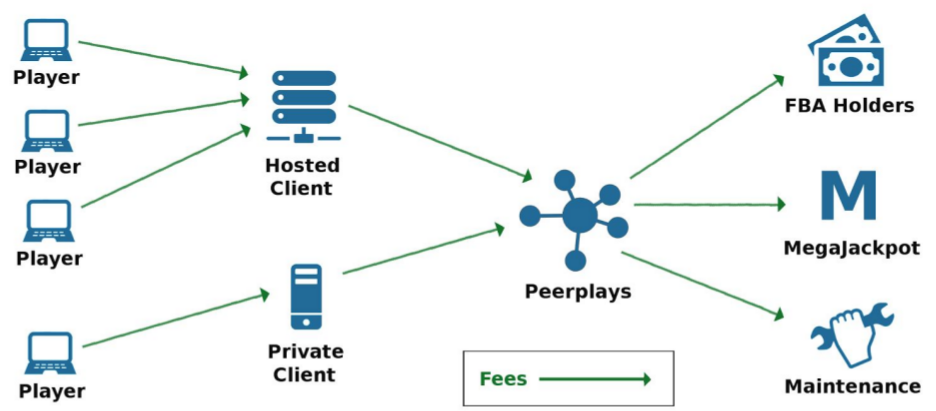
\includegraphics[width=\textwidth]{fig/flowchart}
\end{center}

\section{Mega-Jackpots and PowerUp Points}

Mega-Jackpot tournaments are a way for the Peerplays network to occasionally become the sponsor of large tournament jackpots by utilizing the network’s unique “profit sharing” capabilities. Peerplays automatically allocates a small percentage of every network fee into a smart contract-secured virtual account called the \textit{​Mega-Jackpot Fund}. This smart contract then automatically schedules and hosts Mega-Jackpot tournament events, and the funds are unlocked and instantly transferred to the tournament winners. 

PowerUp points are the user-reward tokens of the Peerplays network, and are distributed according to win-loss records and amounts wagered, among other factors. PowerUp is the only token accepted as the buy-in fee for Mega-Jackpot tournaments, so they will be in high demand during Mega-Jackpot sign up periods. They are tradeable on the asset exchange, andplayers can use them for purchases, rewards, or include them in sponsored Jackpot pools for their own Custom tournaments.

\section{Open Source GUI}

All the operations for regular gameplay on Peerplays will be integrated into a basic open­source Graphic User Interface (GUI) for a seamless user experience. This GUI will be published and maintained, exposing all the basic blockchain functions including simple tools for players to create their own buy­in games, organize and host multi­player tournaments, and buy, sell and create tokens. It will also support live gameplay for all on­chain games. The user interface will be translated into several languages, and will have a modified BSD licence for both personal and commercial use. 

\section{Trustless Asset Exchange}

As a Graphene Blockchain, Peerplays has the same asset creation and exchange features as BitShares,​\cite{9} enabling users to create their own tokens, and place buy and sell orders on the internal market which are filled by the on chain order matching smart contract. They can also transfer, buy and sell gateway tokens for popular cryptocurrencies like BTC and ETH and price-stable \textit{​SmartCoins} from the BitShares platform from a growing number of reputable gateway services. Players can even provide their own profitable gateway services by buying and selling in-game assets for popular RPGs.

\section{Wagering}

The Peerplays tournament smart contract accepts any user issued token for wagering, but charges a small fee if the tokens are not one of the \textit{certified wagering instruments}. These instruments are chosen in accordance with standards of acceptable value as determined by the committee. Certified instruments charge a \textit{rake fee} in place of the standard registration fee, which is automatically distributed as part of the profit sharing program. Users can also place wagers with the Peerplays core token.

\section{Hosted (Public) Client Portals}

Hosted client portals are a way for users to access the Peerplays blockchain through their web browser,​\cite{10} while their private keys are stored locally. They are more convenient than private desktop clients, but like most cryptocurrency wallets they require backups to prevent accidental loss of funds. Private desktop client portals operate much like lightweight wallets that do not require the user to download a full node, but instead reference a series of trusted public nodes. For the highest level of security, users can also run their own full node in conjunction with the desktop client. 

Operating a public hosted client portal is an opportunity for businesses to make extra income through the referral program or by building and connecting an independent 3rd party website to organize and host their own server-side tournaments.

\section{Server-Side Tournament Hosting}

Server-side game hosting is still a trusted and proven model in the eSports industry, and has seen explosive growth in the past 5 years. Peerplays supports optional server-side hosting of games while offering a variety of tools for business enhancement. For example, simply connecting to Peerplays through the API allows anyone to utilize the decentralized network for processing of wagers and jackpots while continuing to operate an independent website. Peerplays’ customizable tournament management smart contract lets any game publisher, advertiser, tournament host or vendor create their own tournament structures, fee schedules, and wager collection & distribution methods for any off-chain (server hosted) game in the world. And gaming partners can offer additional benefits and perks to users by designing their own custom GUI or even by simply hosting the basic open-source Peerplays GUI on a public server. 

Peerplays also has a blockchain guaranteed referral program which automatically pays a percentage of lifetime revenue for each new player referred to the network, which means businesses can earn major “kickbacks” by plugging into Peerplays and getting all their existing users to sign up for a Peerplays account.

\section{Conclusion}

Peerplays offers a unique value proposition to both end users and existing businesses. By combining provably fair gaming with a decentralized blockchain-based wagering, Peerplays effectively tackles several key industry challenges while offering strong incentives for existing gaming platforms to integrate. Overall, the platform is well equipped for future growth and adaptation to changing market conditions due to its next-generation voting and consensus mechanisms, and is strongly positioned to become the premiere go-to provider for blockchain based solutions in the online gaming industry.

\newpage

%%% Bibliography

\begin{thebibliography}{99}
\raggedright
\bibitem{1}
Defunct Poker Sites \url{http://www.pokersites.com/defunct} 
\bibitem{2}
Online Gambling Laws and Jurisdictions \url{http://www.gamblingsites.com/online-gambling-jurisdictions/}
\bibitem{3}
Measuring Performance - Throughput and Latency \url{https://bitshares.org/blog/2015/06/08/measuring-performance/}
\bibitem{4}
The LMAX Architecture \url{http://martinfowler.com/articles/lmax.html}
\bibitem{5}
Industrial Performance and Scalability \url{https://bitshares.org/technology/industrial-performance-and-scalability/}
\bibitem{6}
Decentralized Exchange \url{http://docs.bitshares.org/bitshares/user/dex.html}
\bibitem{7}
Graphene Stress Test Report \url{https://bitsharestalk.org/index.php/topic,18684.0.html}
\bibitem{8}
Fee Backed Assets \url{https://github.com/bitshares/bsips/blob/master/bsip-0007.md}
\bibitem{9}
Assets/Tokens \url{https://docs.bitshares.org/bitshares/user/assets.html}
\bibitem{10}
BitShares GUI (web wallet) \url{https://github.com/bitshares/web_wallet}
\end{thebibliography}

\end{document}
